\documentclass[aspectratio=169, 11pt]{beamer}

% ── Theme: the shared course style of Chapter 1.1 ──
\usetheme{default}
\usepackage[T1]{fontenc}
\usepackage{lmodern}
\usepackage{appendixnumberbeamer}

\usepackage{amsmath, amssymb, amsfonts}
\usepackage{booktabs}
\usepackage{listings}
\usepackage{xcolor}
\usepackage{tikz}
\usetikzlibrary{arrows.meta, positioning, shapes.geometric, fit}
\usepackage{graphicx}
\usepackage{multicol}
\graphicspath{{experiments/figures/}}

% ── Course colours and slide layout (as in Chapter 1.1) ──
\definecolor{FEMnavy}{HTML}{17365D}
\definecolor{FEMblue}{HTML}{2B6CB0}
\definecolor{FEMteal}{HTML}{1597A5}
\definecolor{FEMorange}{HTML}{D7653B}
\definecolor{FEMlight}{HTML}{F4F7FA}
\definecolor{FEMgray}{HTML}{5C6F82}
\definecolor{FEMpale}{HTML}{EAF7F9}
\definecolor{FEMcream}{HTML}{FFF4EA}
\setbeamercolor{normal text}{fg=FEMnavy,bg=white}
\setbeamercolor{structure}{fg=FEMblue}
\setbeamercolor{frametitle}{fg=white,bg=FEMnavy}
\setbeamercolor{title}{fg=white}
\setbeamercolor{block title}{fg=white,bg=FEMblue}
\setbeamercolor{block body}{fg=FEMnavy,bg=FEMlight}
\setbeamercolor{alerted text}{fg=FEMorange}
\setbeamercolor{block title alerted}{fg=white,bg=FEMorange}
\setbeamercolor{block body alerted}{fg=FEMnavy,bg=FEMcream}
\setbeamercolor{block title example}{fg=white,bg=FEMteal}
\setbeamercolor{block body example}{fg=FEMnavy,bg=FEMpale}
\setbeamertemplate{navigation symbols}{}
\setbeamertemplate{itemize item}{\color{FEMteal}$\blacktriangleright$}
\setbeamertemplate{itemize subitem}{\color{FEMteal}$\bullet$}
\setbeamertemplate{frametitle}{\nointerlineskip\begin{beamercolorbox}[wd=\paperwidth,ht=.82cm,dp=.25cm,leftskip=.55cm]{frametitle}\usebeamerfont{frametitle}\insertframetitle\end{beamercolorbox}}
\setbeamertemplate{footline}{\leavevmode\hbox{\begin{beamercolorbox}[wd=.82\paperwidth,ht=2.6ex,dp=1.1ex,leftskip=.55cm]{author in head/foot}\color{FEMgray}\scriptsize Introduction to FEniCS -- Part II\end{beamercolorbox}\begin{beamercolorbox}[wd=.18\paperwidth,ht=2.6ex,dp=1.1ex,rightskip=.55cm plus1fil]{date in head/foot}\color{FEMgray}\scriptsize\hfill\insertframenumber/\inserttotalframenumber\end{beamercolorbox}}}
\setbeamersize{text margin left=.65cm,text margin right=.65cm}
\setbeamerfont{frametitle}{size=\Large,series=\bfseries}
\setbeamerfont{block title}{size=\normalsize,series=\bfseries}

% Title and divider slides in the style of the Chapter 1.1 title page.
\newcommand{\meshmotif}{%
\begin{scope}[shift={(current page.south east)},x=1cm,y=1cm]
\foreach \x in {-6,-4.7,-3.4,-2.1,-.8}{\foreach \y in {.1,1.4,2.7,4,5.3,6.6}{
\draw[white,opacity=.10] (\x,\y) rectangle ++(1.3,1.3);
\draw[white,opacity=.10] (\x,\y)--++(1.3,1.3);}}
\end{scope}}
% #1 kicker line, #2 bottom line
\newcommand{\coursetitleframe}[2]{%
\begin{frame}[plain]
\begin{tikzpicture}[remember picture,overlay]
\fill[FEMnavy] (current page.south west) rectangle (current page.north east);
\meshmotif
\node[anchor=west,text width=12.7cm,align=left] at ([xshift=.85cm,yshift=.55cm]current page.west) {
{\color{FEMteal!70!white}\large\bfseries #1}\\[7mm]
{\color{white}\fontsize{29}{34}\selectfont\bfseries\inserttitle}\\[5mm]
{\color{white!80}\Large\insertsubtitle}\\[6mm]
{\color{white!70}\large\insertauthor}};
\node[anchor=south west,text=white!70] at ([xshift=.85cm,yshift=.72cm]current page.south west) {#2};
\end{tikzpicture}
\end{frame}}
% #1 kicker line (may be empty), #2 title
\newcommand{\dividerframe}[2]{%
\begin{frame}[plain]
\begin{tikzpicture}[remember picture,overlay]
\fill[FEMnavy] (current page.south west) rectangle (current page.north east);
\meshmotif
\node[anchor=west,text width=12.7cm,align=left] at ([xshift=.85cm]current page.west) {
\ifx\relax#1\relax\else{\color{FEMteal!70!white}\large\bfseries #1}\\[6mm]\fi
{\color{white}\fontsize{26}{31}\selectfont\bfseries\hyphenpenalty=10000\exhyphenpenalty=10000 #2\par}};
\end{tikzpicture}
\end{frame}}

% Code listing style, matching Part I
\colorlet{codebg}{FEMlight}
\definecolor{codegreen}{HTML}{2E7D32}
\colorlet{codeapi}{FEMteal!85!black}   % FEniCS/UFL names
\colorlet{codeorange}{FEMorange}
\colorlet{codegray}{FEMgray}
\colorlet{codeblue}{FEMblue}

\lstdefinestyle{fenics}{
    language=Python,
    backgroundcolor=\color{codebg},
    basicstyle=\ttfamily\scriptsize,
    keywordstyle=\color{codeblue}\bfseries,
    stringstyle=\color{codegreen},
    commentstyle=\color{codegray}\itshape,
    emphstyle=\color{codeapi}\bfseries,
    emph={FunctionSpace, TrialFunction, TestFunction, Function,
          DirichletBC, Expression, Constant, UnitSquareMesh,
          UnitCubeMesh, VectorFunctionSpace, NonlinearVariationalProblem,
          NonlinearVariationalSolver, MixedElement, FiniteElement,
          NonlinearProblem, LinearProblem, solve, assemble, plot,
          errornorm, project, derivative, interpolate, grad, div, dot,
          inner, dx, ds},
    morekeywords={[2]mesh, V, W, u, v, p, q, a, L, F, J, bc, f, u_h, y, y_n},
    keywordstyle={[2]\color{codeorange}},
    numbers=left,
    numberstyle=\tiny\color{codegray},
    numbersep=5pt,
    frame=single,
    rulecolor=\color{FEMblue!20},
    breaklines=true,
    showstringspaces=false,
    tabsize=4,
    xleftmargin=6pt,
    xrightmargin=4pt,
    aboveskip=6pt,
    belowskip=4pt,
}

\lstset{style=fenics}

% Metadata
\title{Introduction to FEniCS}
\subtitle{Advanced PDE examples}
\author{Daniel Fernandez}
\date{}

\begin{document}

\coursetitleframe{FINITE ELEMENTS IN PRACTICE\enspace$\cdot$\enspace PART II}{Nonlinear\quad$\cdot$\quad nonlocal\quad$\cdot$\quad optimal control\quad$\cdot$\quad coupled systems}

% --------------------------------------------------------------------------
\section{Roadmap}
% --------------------------------------------------------------------------

\begin{frame}{What changes in Part II}

We still write a weak form, discretize, and solve. Here the equations
add nonlinear coefficients, nonlocal terms, controls, and coupled fields.

\begin{enumerate}
    \item Nonlinear elliptic operator: 3D $p$-Laplacian
    \item Nonlocal parabolic coefficient: diffusion depends on $\int_\Omega u$
    \item Degenerate nonlocal null control: compute a source on $\omega$
    \item PDE-constrained optimization: state, adjoint, and control
    \item Coupled nonlinear systems: reaction-diffusion pattern formation
\end{enumerate}

\end{frame}

\begin{frame}[fragile]{Start with the residual}

\begin{columns}[T]
\column{0.48\textwidth}
\textbf{Mathematics}
\[
    F(u;v)=0
    \qquad \forall v \in V
\]

\[
    J(u;\delta u,v)
    =
    \frac{d}{d\epsilon}
    F(u+\epsilon\delta u;v)\big|_{\epsilon=0}
\]

\column{0.50\textwidth}
\textbf{FEniCSx}
\begin{lstlisting}[basicstyle=\ttfamily\tiny]
u = fem.Function(V)
v = ufl.TestFunction(V)

F = ...                 # residual
J = ufl.derivative(F, u)

problem = NonlinearProblem(
    F, u, bcs=[bc], J=J)
problem.solve()
\end{lstlisting}
\end{columns}

\end{frame}

% --------------------------------------------------------------------------
\section{3D p-Laplacian}
% --------------------------------------------------------------------------

\dividerframe{EXAMPLE 7}{3D $p$-Laplacian}

\begin{frame}{A porous-flow model in three dimensions}

\begin{block}{Pressure-driven flow of a power-law fluid in a porous block}
\[
 -\nabla \cdot
 \left(
    K(x)
    \bigl(\varepsilon^2 + |\nabla u|^2\bigr)^{\frac{p-2}{2}}
    \nabla u
 \right)
 + \sigma u = s(x)
 \quad \text{in } \Omega=(0,1)^3
\]
\[
    K(x)
    \bigl(\varepsilon^2 + |\nabla u|^2\bigr)^{\frac{p-2}{2}}
    \nabla u\cdot n = 0
    \quad \text{on } \partial\Omega.
\]
\end{block}

\medskip
\small
\begin{itemize}
    \item $u$: pressure head or hydraulic head in the 3D block.
    \item $-K(\varepsilon^2+|\nabla u|^2)^{(p-2)/2}\nabla u$: nonlinear flux.
    \item $K(x)$: heterogeneous permeability of the medium.
    \item $s(x)$: injection/extraction wells or volumetric forcing.
    \item $\sigma u$: small leakage/reference term for the Neumann model.
    \item $p=2$: linear Darcy/Poisson model; $p\neq2$: power-law rheology.
\end{itemize}

\end{frame}

\begin{frame}{Weak form}

Let $V=H^1(\Omega)$ and define
\[
    \mu(\nabla u)
    =
    \bigl(\varepsilon^2+|\nabla u|^2\bigr)^{\frac{p-2}{2}}.
\]

\medskip
Find $u\in V$ such that
\[
    F(u;v)
    =
    \int_\Omega
        K(x)\,\mu(\nabla u)\,\nabla u\cdot\nabla v\,dx
    +
    \int_\Omega \sigma u\,v\,dx
    -
    \int_\Omega s\,v\,dx
    =
    0
    \quad \forall v\in V.
\]

\bigskip
\small
\textbf{Regularization:}
$\varepsilon>0$ regularizes the operator near $|\nabla u|=0$.
The demo uses $p=3$ and homogeneous Neumann data.  The $\sigma u$ term fixes
the additive constant that a pure Neumann operator would otherwise leave free.

\end{frame}

\begin{frame}[fragile,shrink=6]{p-Laplacian: key code}

\begin{lstlisting}[basicstyle=\ttfamily\tiny]
msh = mesh.create_unit_cube(MPI.COMM_WORLD, 14, 14, 14)
V = fem.functionspace(msh, ("Lagrange", 1))

u = fem.Function(V, name="u")
v = ufl.TestFunction(V)
x = ufl.SpatialCoordinate(msh)

K = 0.7 + 0.6*x[2] + 0.15*ufl.sin(2.0*ufl.pi*x[0])
source = injection_well(x) - extraction_well(x)
sigma = 0.15

grad_u = ufl.grad(u)
mobility = (eps**2 + ufl.inner(grad_u, grad_u))**((p_exp-2.0)/2.0)

F = K*mobility*ufl.inner(grad_u, ufl.grad(v))*ufl.dx \
    + sigma*u*v*ufl.dx \
    - source*v*ufl.dx
J = ufl.derivative(F, u)

problem = NonlinearProblem(F, u, bcs=[], J=J,
    petsc_options={"snes_type": "newtonls",
                   "ksp_type": "preonly", "pc_type": "lu"})
problem.solve()
\end{lstlisting}

\vspace{-0.4em}
\scriptsize
\texttt{snes\_type=newtonls}: Newton with line search.
\texttt{ksp\_type=preonly, pc\_type=lu}: solve each Newton linear system directly by LU.

\end{frame}

\begin{frame}{p-Laplacian: 3D result}

\begin{center}
    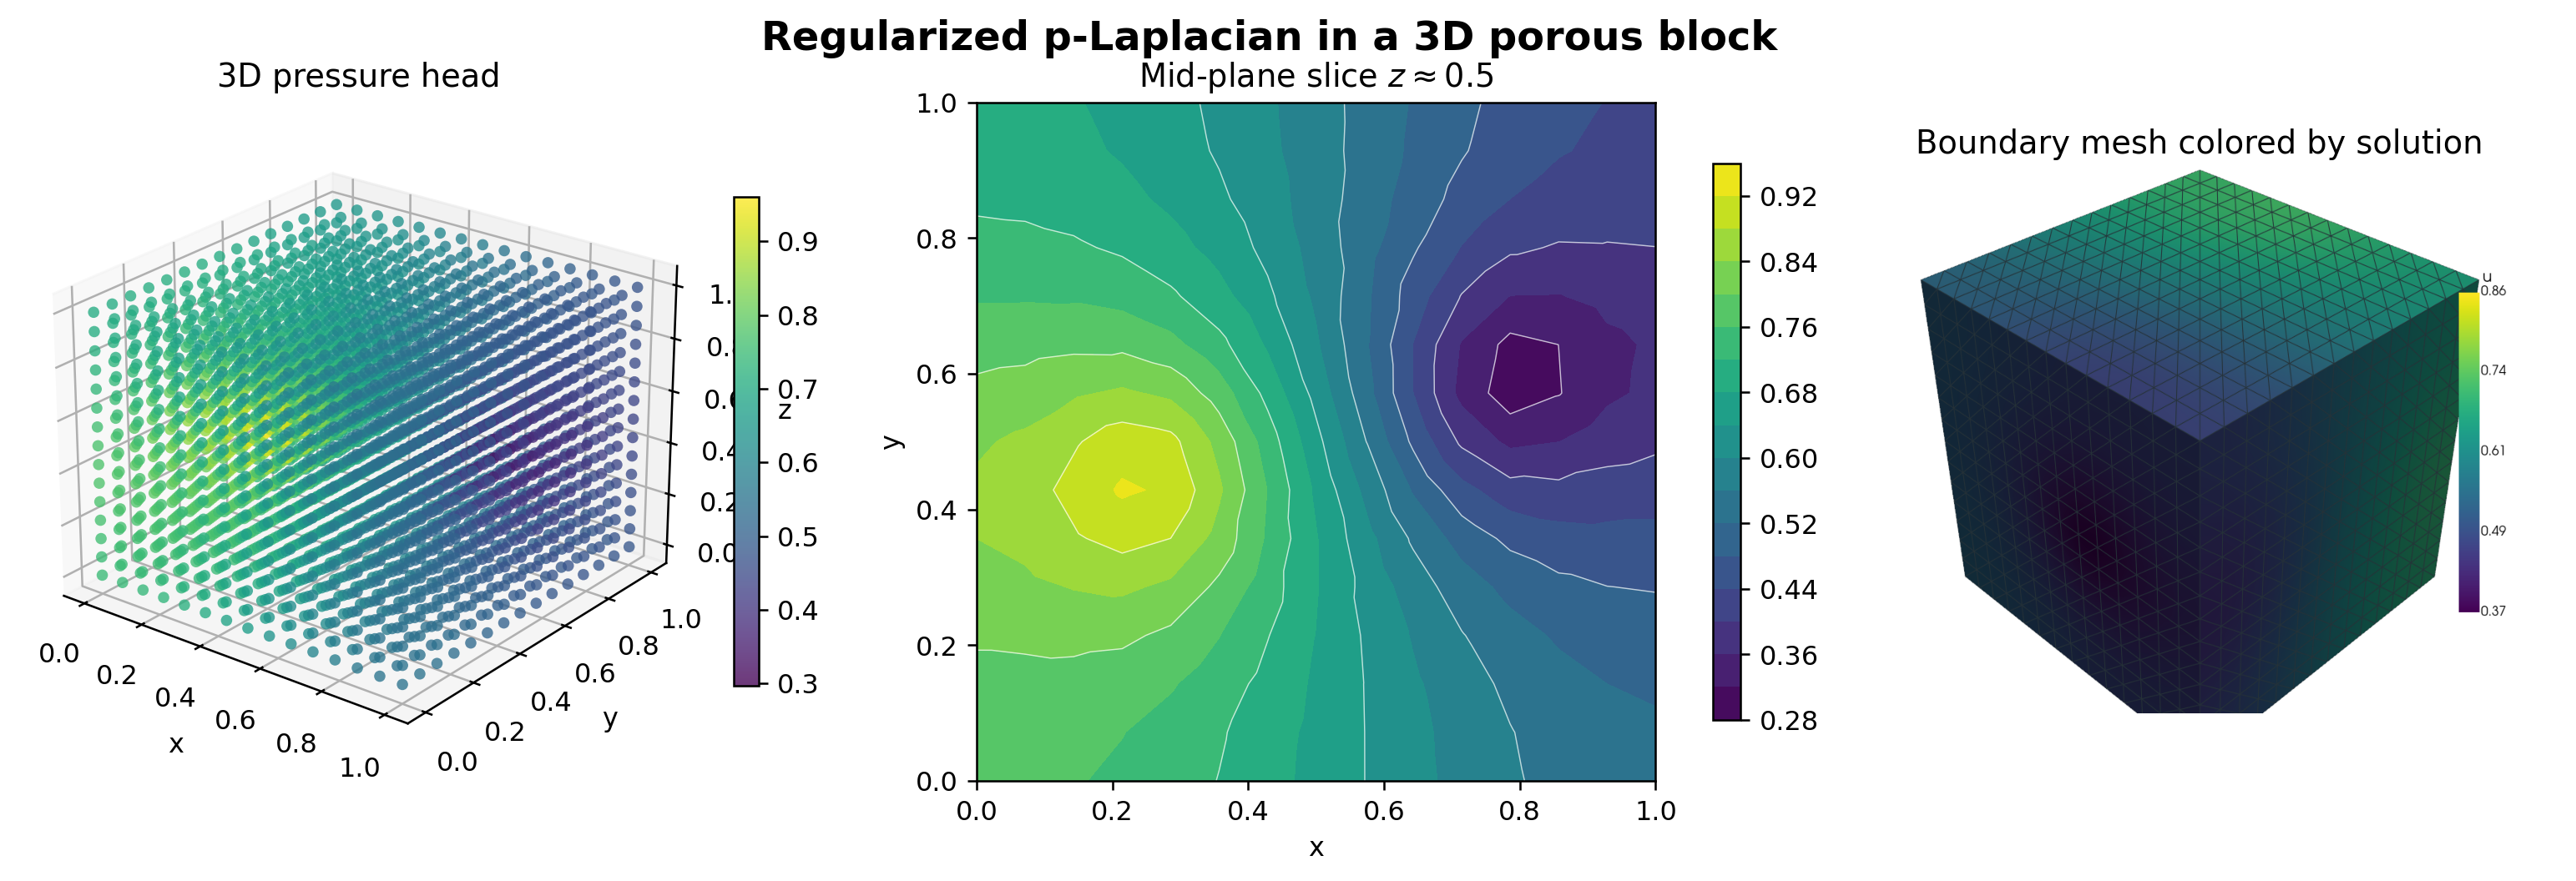
\includegraphics[width=\textwidth,height=0.82\textheight,keepaspectratio]{p_laplacian_3d.png}
\end{center}

\end{frame}

% --------------------------------------------------------------------------
\section{Nonlocal parabolic PDE}
% --------------------------------------------------------------------------

\dividerframe{EXAMPLE 8}{Nonlocal parabolic PDE}

\begin{frame}{Nonlocal state equation}

\begin{block}{Problem}
\[
    u_t -
    \left(
        a(x)
        \int_\Omega u(\xi,t)\,d\xi
        \,u_x
    \right)_x
    =
    h(x)\mathbf{1}_O(x),
    \qquad
    \Omega=(0,1),\quad t\in(0,T).
\]
\[
    u(0,t)=u(1,t)=0,
    \qquad
    u(x,0)=y_0(x).
\]
\end{block}

\medskip
\small
\begin{itemize}
    \item $M(t)=\int_0^1 u(x,t)\,dx$ couples every point to the global state.
    \item $a(x)$ is the local transport/diffusion profile.
    \item $h(x)\mathbf{1}_O$ is an actuator or forcing active only on $O$.
    \item Demo choice: $O=(0.35,0.65)$ and several pairs $(a,h)$.
\end{itemize}

\end{frame}

\begin{frame}{Backward Euler + Picard linearization}

Let $M^{n+1}=\int_0^1 u^{n+1}(x)\,dx$.
For $v\in H_0^1(0,1)$,
\[
    (u^{n+1},v)
    + \Delta t\,M^{n+1}\,(a\,u_x^{n+1},v_x)
    =
    (u^n,v)
    + \Delta t\,(h\mathbf{1}_O,v).
\]

\bigskip
\textbf{Picard loop at each time step:}
\[
    M_k = \int_0^1 u_k^{n+1}\,dx,
    \qquad
    (u_{k+1}^{n+1},v)
    + \Delta t\,M_k(a(u_{k+1}^{n+1})_x,v_x)
    =
    (u^n,v)+\Delta t(h\mathbf{1}_O,v).
\]

\medskip
\small
This turns the nonlocal nonlinear step into repeated linear variational solves.

\end{frame}

\begin{frame}[fragile]{Nonlocal PDE: key code}

\begin{lstlisting}[basicstyle=\ttfamily\tiny]
u = ufl.TrialFunction(V)
v = ufl.TestFunction(V)
M = fem.Constant(msh, default_scalar_type(0.0))
dt = fem.Constant(msh, default_scalar_type(DT))
a_form = u*v*ufl.dx \
    + dt*M*a_fun*ufl.dot(ufl.grad(u), ufl.grad(v))*ufl.dx
L_form = u_n*v*ufl.dx + dt*h_fun*v*ufl.dx
problem = LinearProblem(a_form, L_form, bcs=[bc],
    petsc_options={"ksp_type": "preonly", "pc_type": "lu"})

for step in range(1, num_steps + 1):
    mass_k = assemble_integral(u_n)
    u_picard = fem.Function(V)
    u_picard.x.array[:] = u_n.x.array
    for k in range(max_picard):
        M.value = default_scalar_type(mass_k)
        u_new = problem.solve()   # one linear solve per Picard step
        mass_new = assemble_integral(u_new)
        update = max(abs(u_new.x.array - u_picard.x.array))
        if update < update_tol and abs(mass_new - mass_k) < mass_tol:
            break
        u_picard.x.array[:] = u_new.x.array; mass_k = mass_new
    u_n.x.array[:] = u_new.x.array
\end{lstlisting}

\end{frame}

\begin{frame}{Nonlocal PDE: tested choices of $a$ and $h$}

\small
\begin{center}
\renewcommand{\arraystretch}{1.25}
\begin{tabular}{lll}
\toprule
\textbf{Case} & \textbf{$a(x)$} & \textbf{$h(x)$ on $O$} \\
\midrule
Uniform & $0.28$ & $1.15$ \\
Oscillatory & $0.22(1+0.55\sin(2\pi x))+0.04$
             & $1.25(1+0.60\cos(2\pi x))$ \\
Layered & $0.08+\dfrac{0.34}{1+\exp(-45(x-0.58))}$
        & $2\exp(-95(x-0.48)^2)$ \\
\bottomrule
\end{tabular}
\end{center}

\end{frame}

\begin{frame}{Nonlocal PDE: varying $a$ and $h$}

\begin{center}
    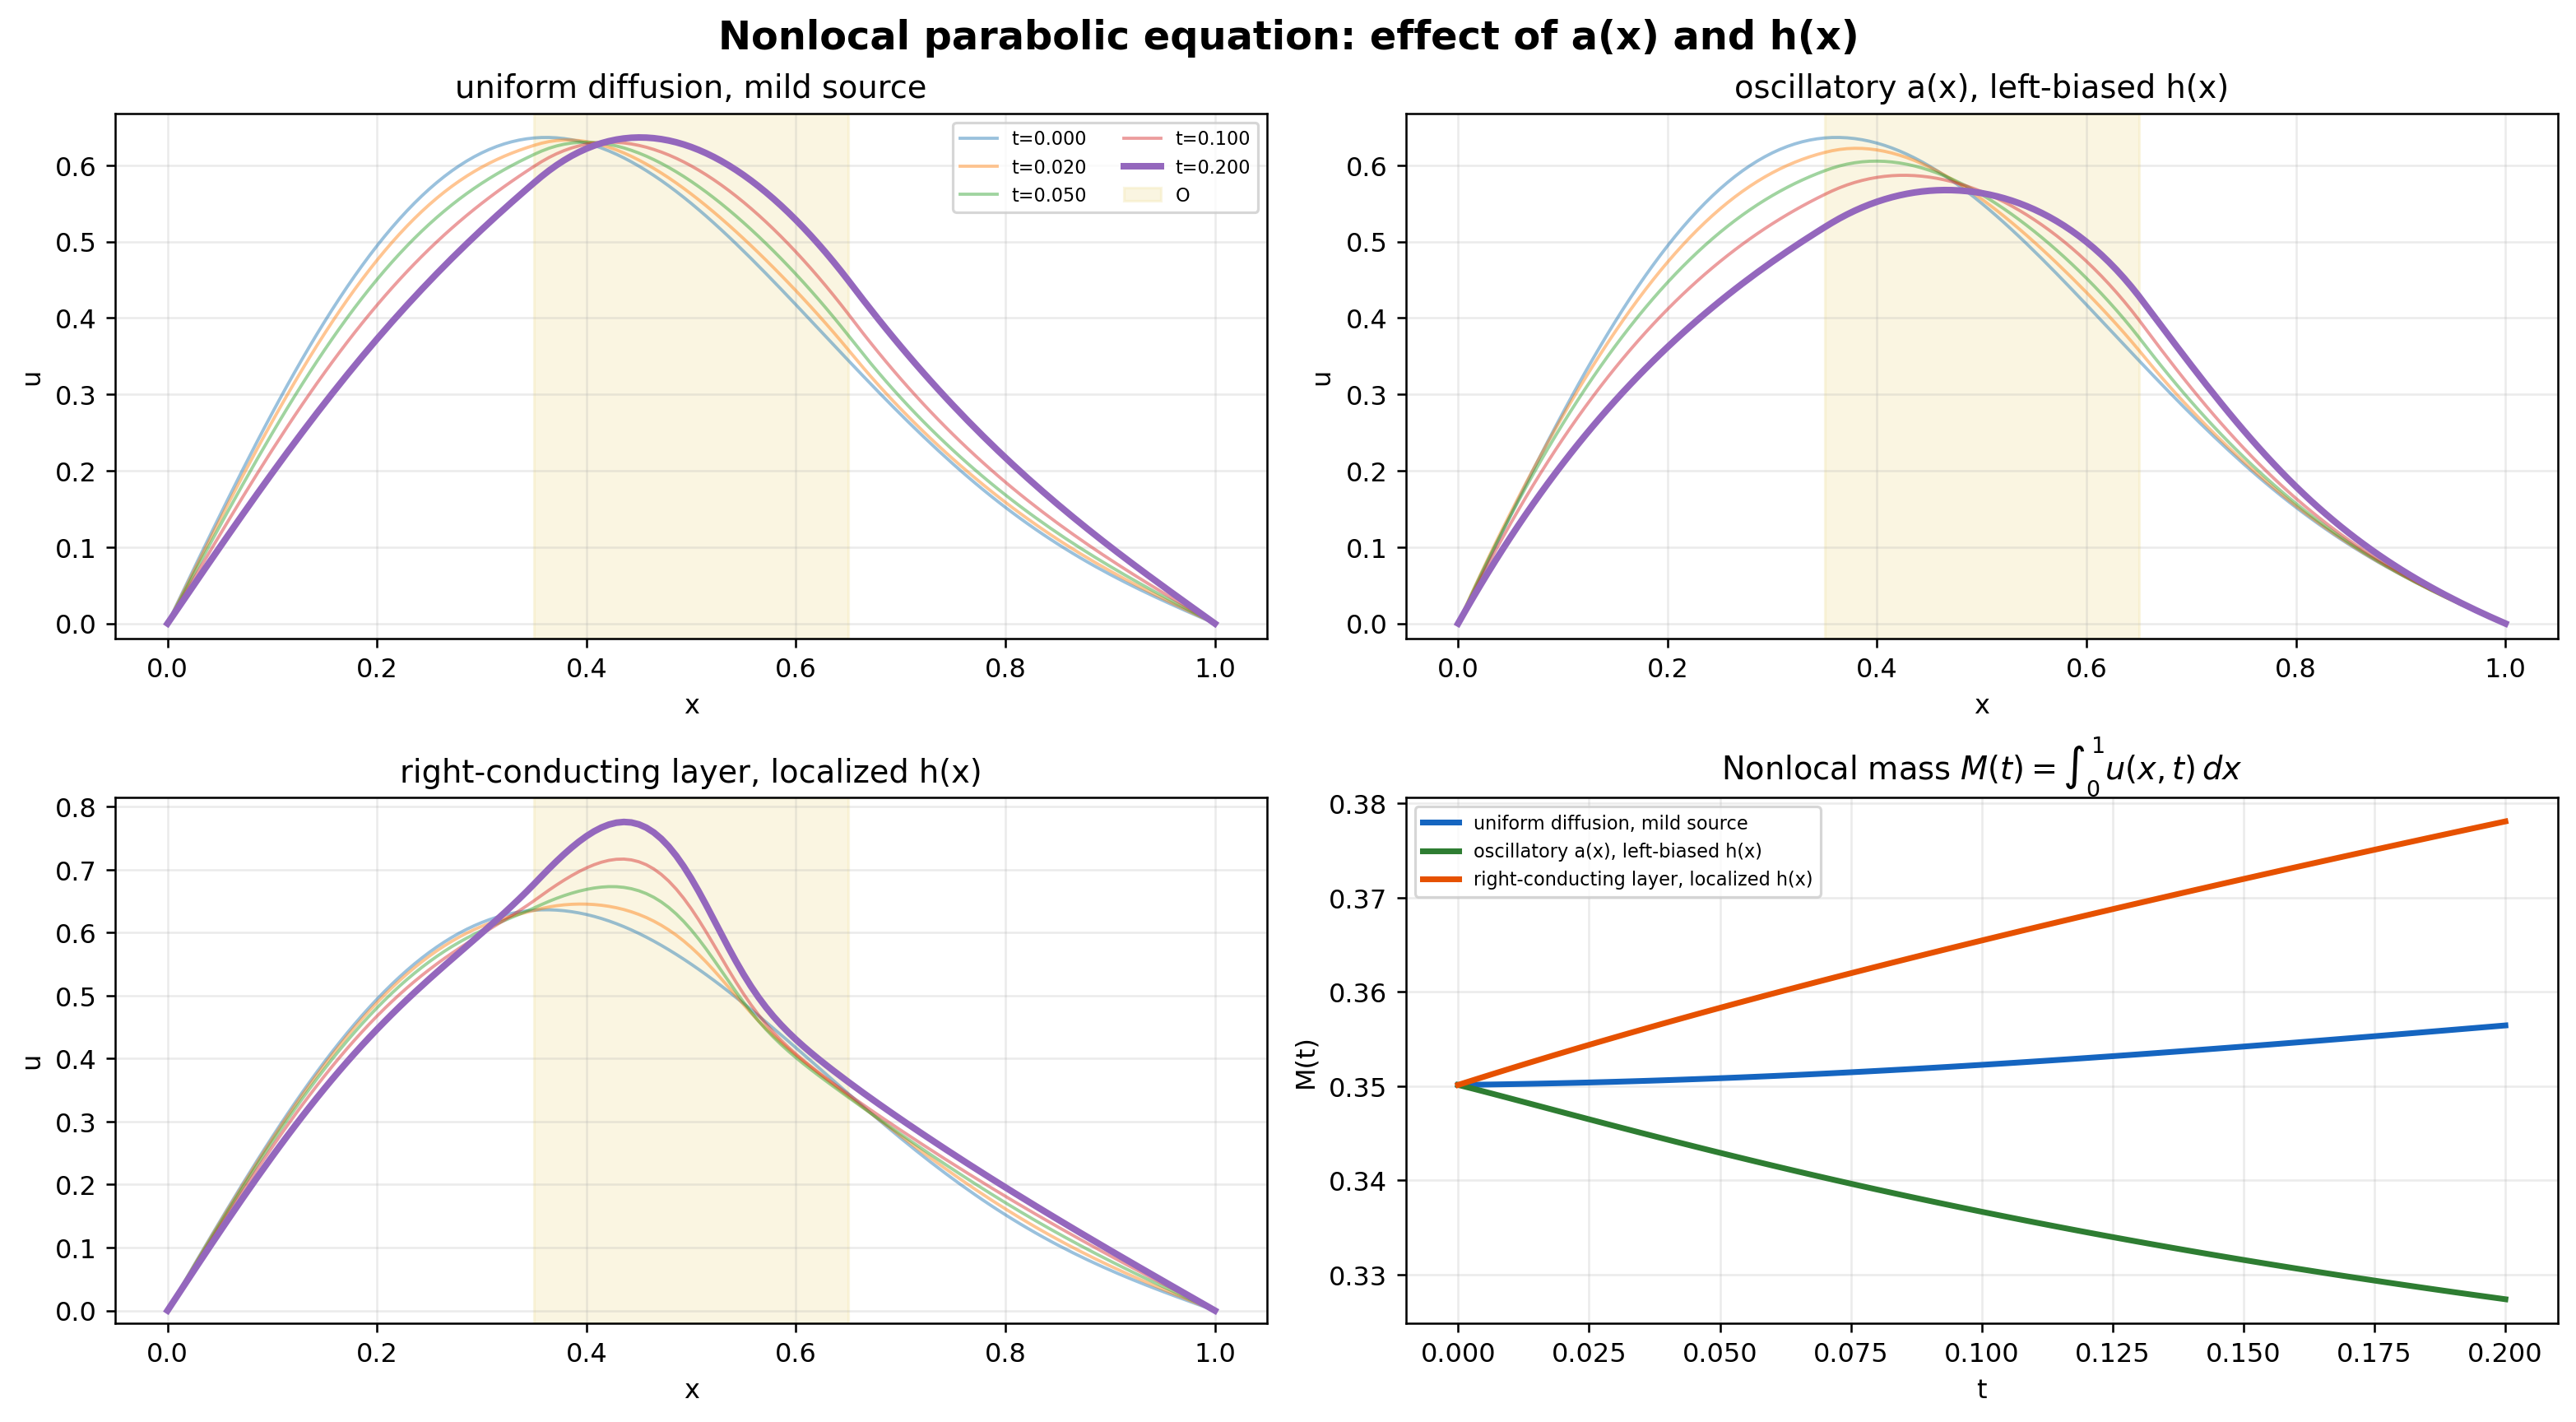
\includegraphics[width=\textwidth,height=0.82\textheight,keepaspectratio]{nonlocal_variants.png}
\end{center}

\end{frame}

% --------------------------------------------------------------------------
\section{Degenerate nonlocal null control}
% --------------------------------------------------------------------------

\dividerframe{EXAMPLE 9}{Degenerate nonlocal null control}

\begin{frame}{Degenerate nonlocal state equation}

\begin{block}{Controlled equation}
\[
\begin{aligned}
    u_t
    - \ell\!\left(\int_0^1 u(x,t)\,dx\right)
      \bigl(x^\gamma u_x\bigr)_x
    -20t\,u
    &=
    h(t,x)\mathbf{1}_\omega(x),
    \qquad (t,x)\in(0,T)\times(0,1),\\
    u(0,x) &= 2\sin(2\pi x),
    \qquad
    \ell(r)=1+\frac{1}{1+r^2}.
\end{aligned}
\]
\end{block}

\medskip
\small
\begin{itemize}
    \item $\gamma\in\{0.5,1,1.5\}$ controls the strength of degeneracy at $x=0$.
    \item Weak case $\gamma<1$: $u(t,0)=u(t,1)=0$.
    \item Strong case $\gamma\ge 1$: $(x^\gamma u_x)(t,0)=0$ and $u(t,1)=0$.
    \item The goal is to choose $h$ on $\omega$ so that $u(T)\approx0$.
\end{itemize}

\end{frame}

\begin{frame}{Control domains and numerical loop}

\small
\begin{center}
\renewcommand{\arraystretch}{1.18}
\begin{tabular}{ccc}
\toprule
\textbf{Domain} & $\boldsymbol{\omega}$ & $\boldsymbol{\omega'}$ \\
\midrule
1 & $(0.2,0.8)$ & $(0.21,0.79)$ \\
2 & $(0.2,0.8)$ & $(0.3,0.7)$ \\
3 & $(0.4,0.6)$ & $(0.42,0.58)$ \\
\bottomrule
\end{tabular}
\end{center}

\medskip
\begin{enumerate}
    \item Backward Euler in time and finite differences in space.
    \item Newton solves the fully nonlinear time step, including the derivative of $\ell(\int u)$.
    \item A frozen linear null control is computed from the discrete controllability map.
    \item A discrete adjoint refinement reduces the nonlinear terminal error.
\end{enumerate}

\medskip
\small
Run: $T=1$, a feature-refined spatial grid with $60$ target intervals, and
$120$ time steps. Nodes cluster near $x=0$ and the interfaces of
$\omega,\omega'$.

\end{frame}

\begin{frame}{3D surface with mesh: $\gamma=0.5$}

\begin{center}
    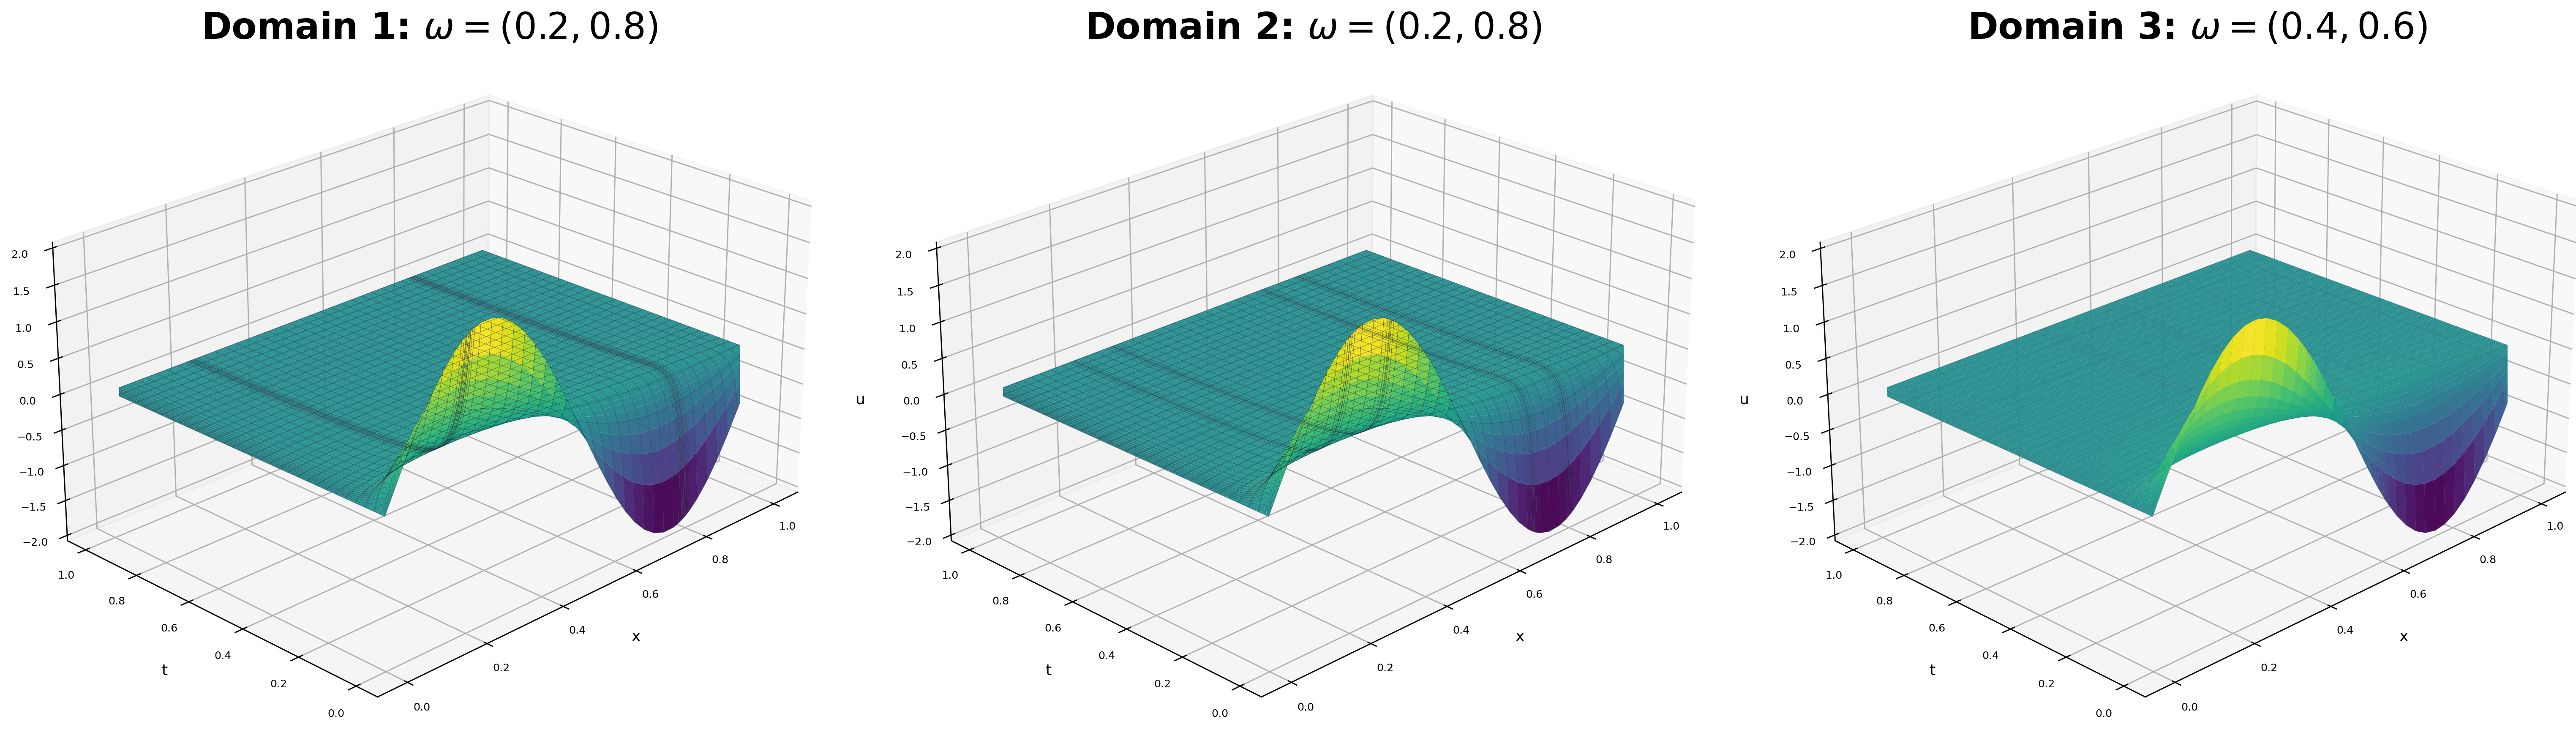
\includegraphics[width=\textwidth,height=0.80\textheight,keepaspectratio,trim=0 18bp 0 0,clip]{degenerate_nonlocal_control_surface_gamma05.png}
\end{center}

\end{frame}

\begin{frame}{3D surface with mesh: $\gamma=1$}

\begin{center}
    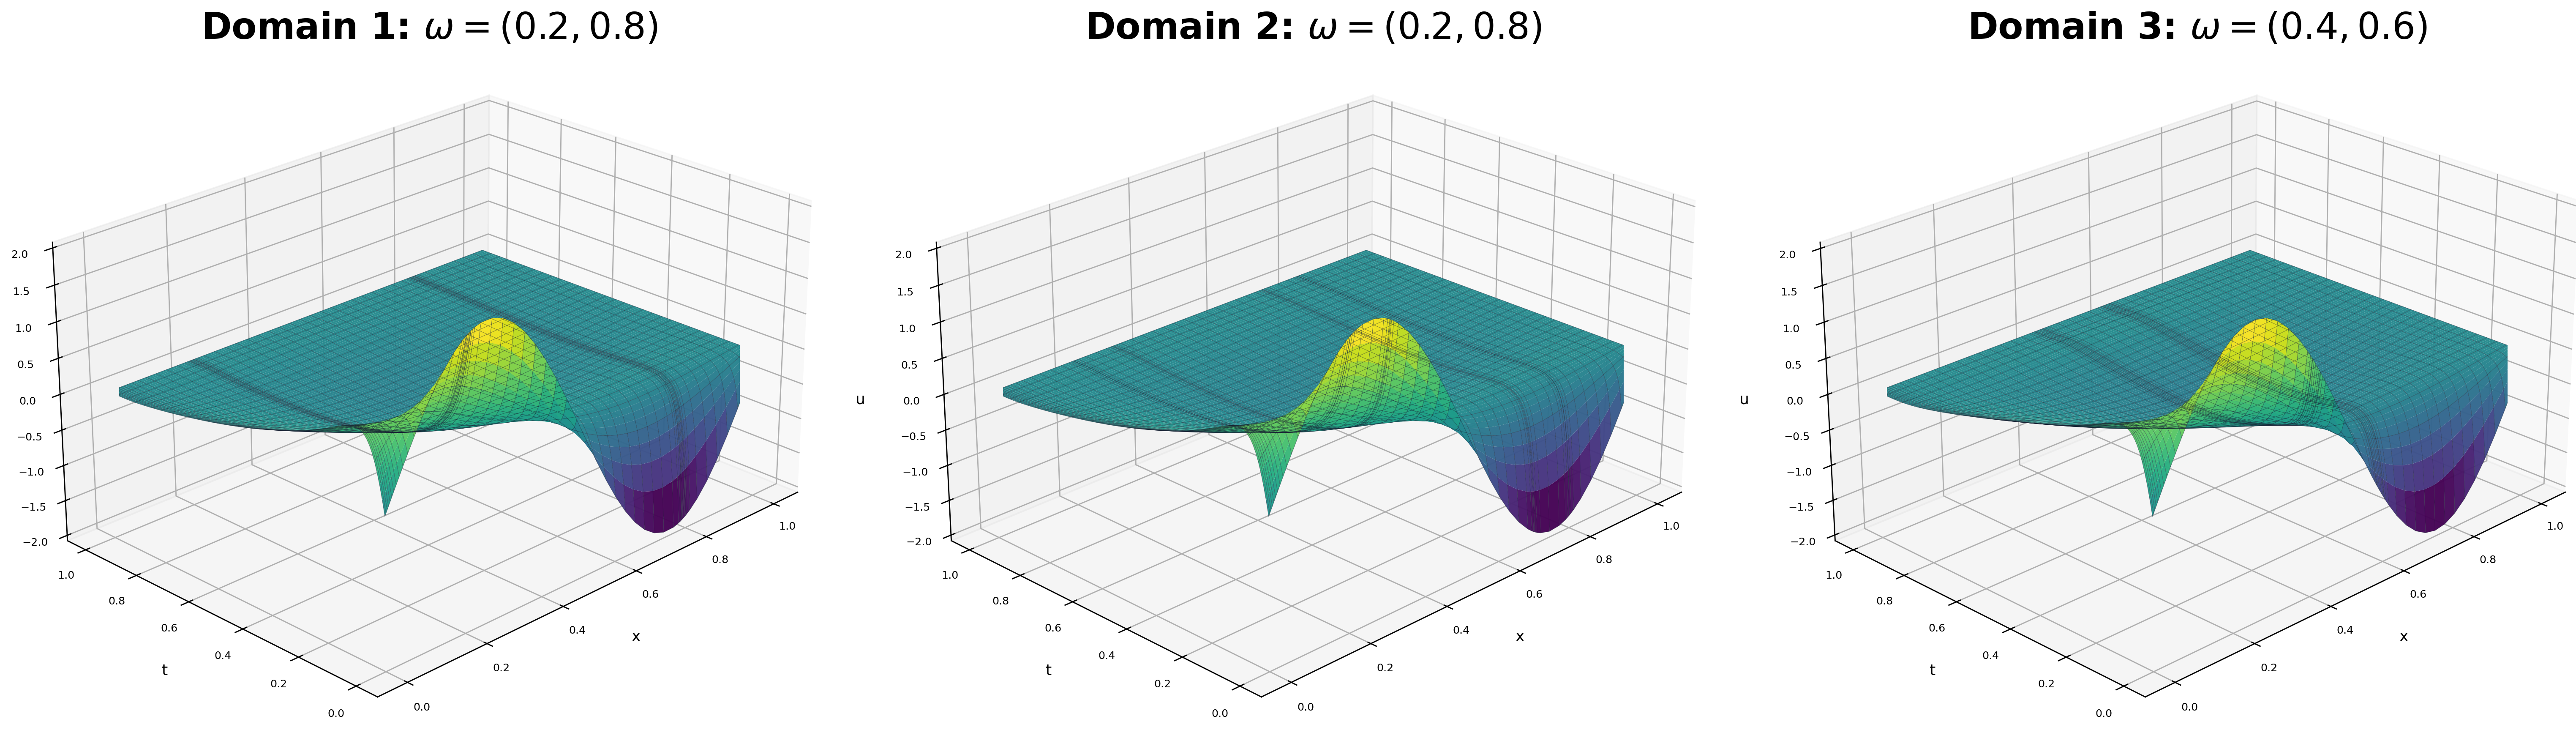
\includegraphics[width=\textwidth,height=0.80\textheight,keepaspectratio,trim=0 18bp 0 0,clip]{degenerate_nonlocal_control_surface_gamma10.png}
\end{center}

\end{frame}

\begin{frame}{3D surface with mesh: $\gamma=1.5$}

\begin{center}
    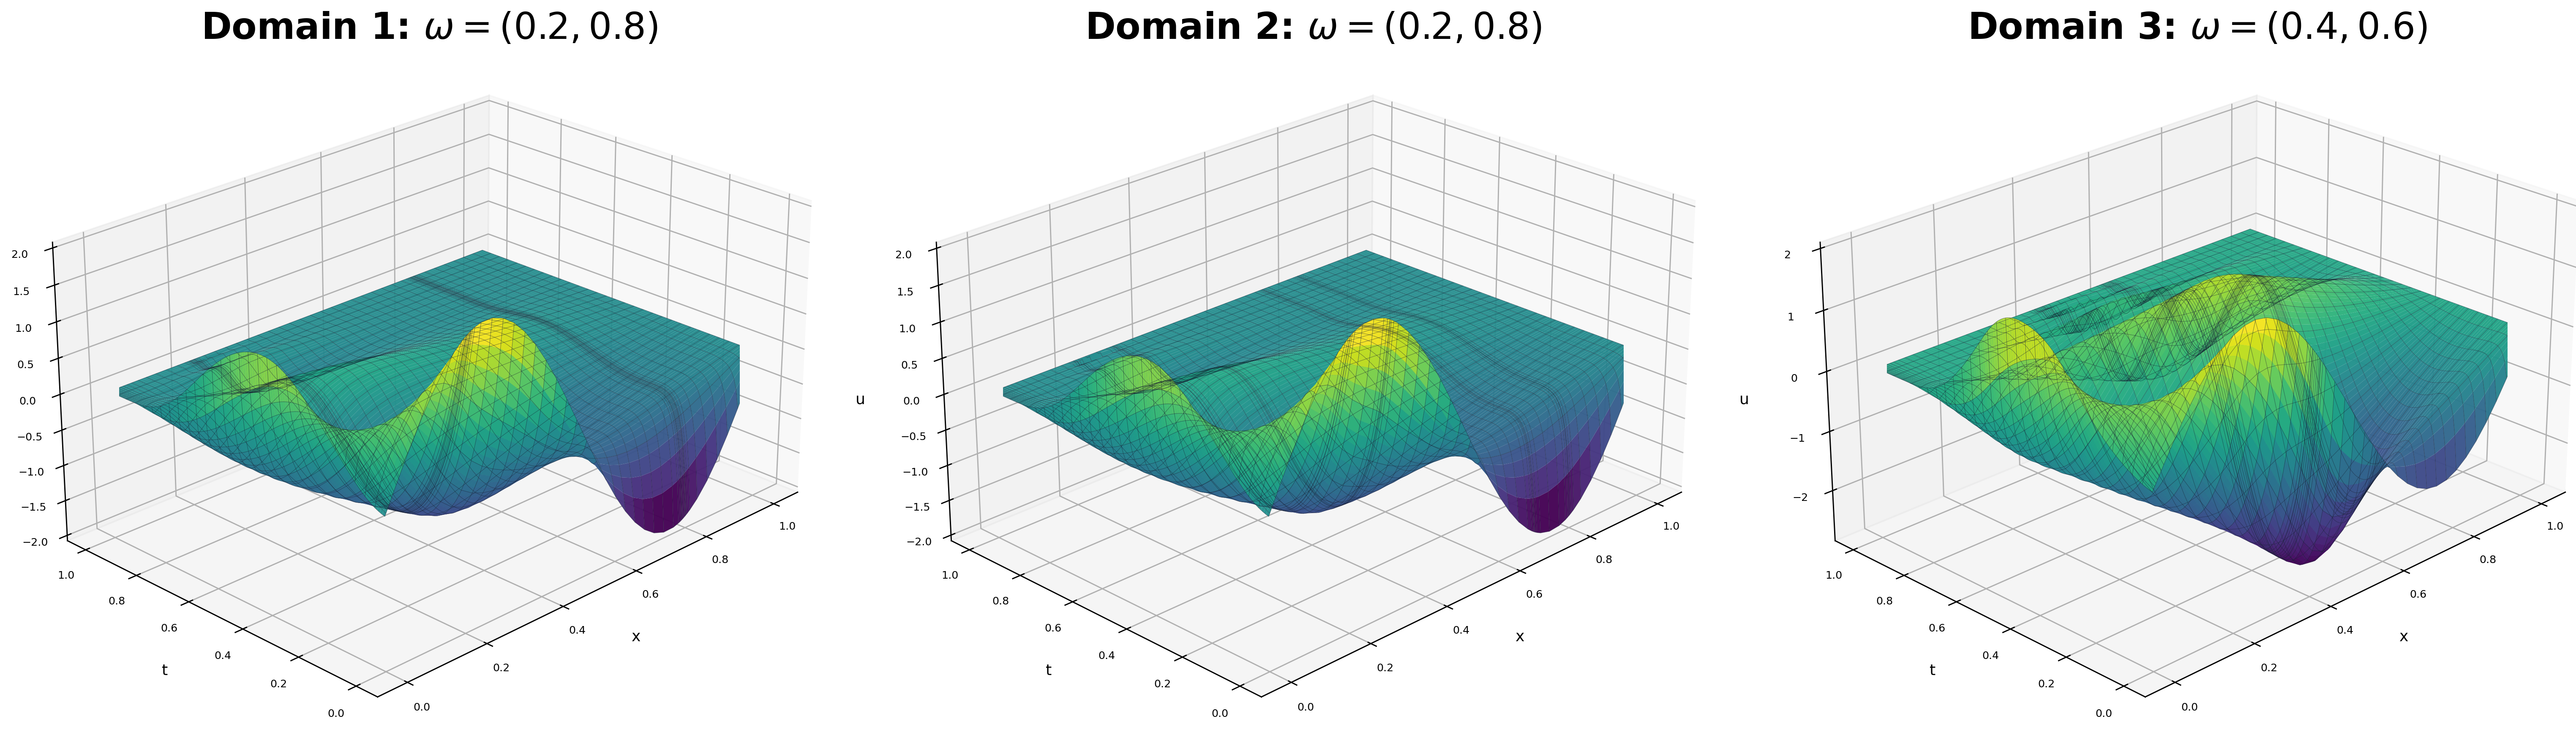
\includegraphics[width=\textwidth,height=0.80\textheight,keepaspectratio,trim=0 18bp 0 0,clip]{degenerate_nonlocal_control_surface_gamma15.png}
\end{center}

\end{frame}

\begin{frame}{3D visualization variants}

\begin{center}
    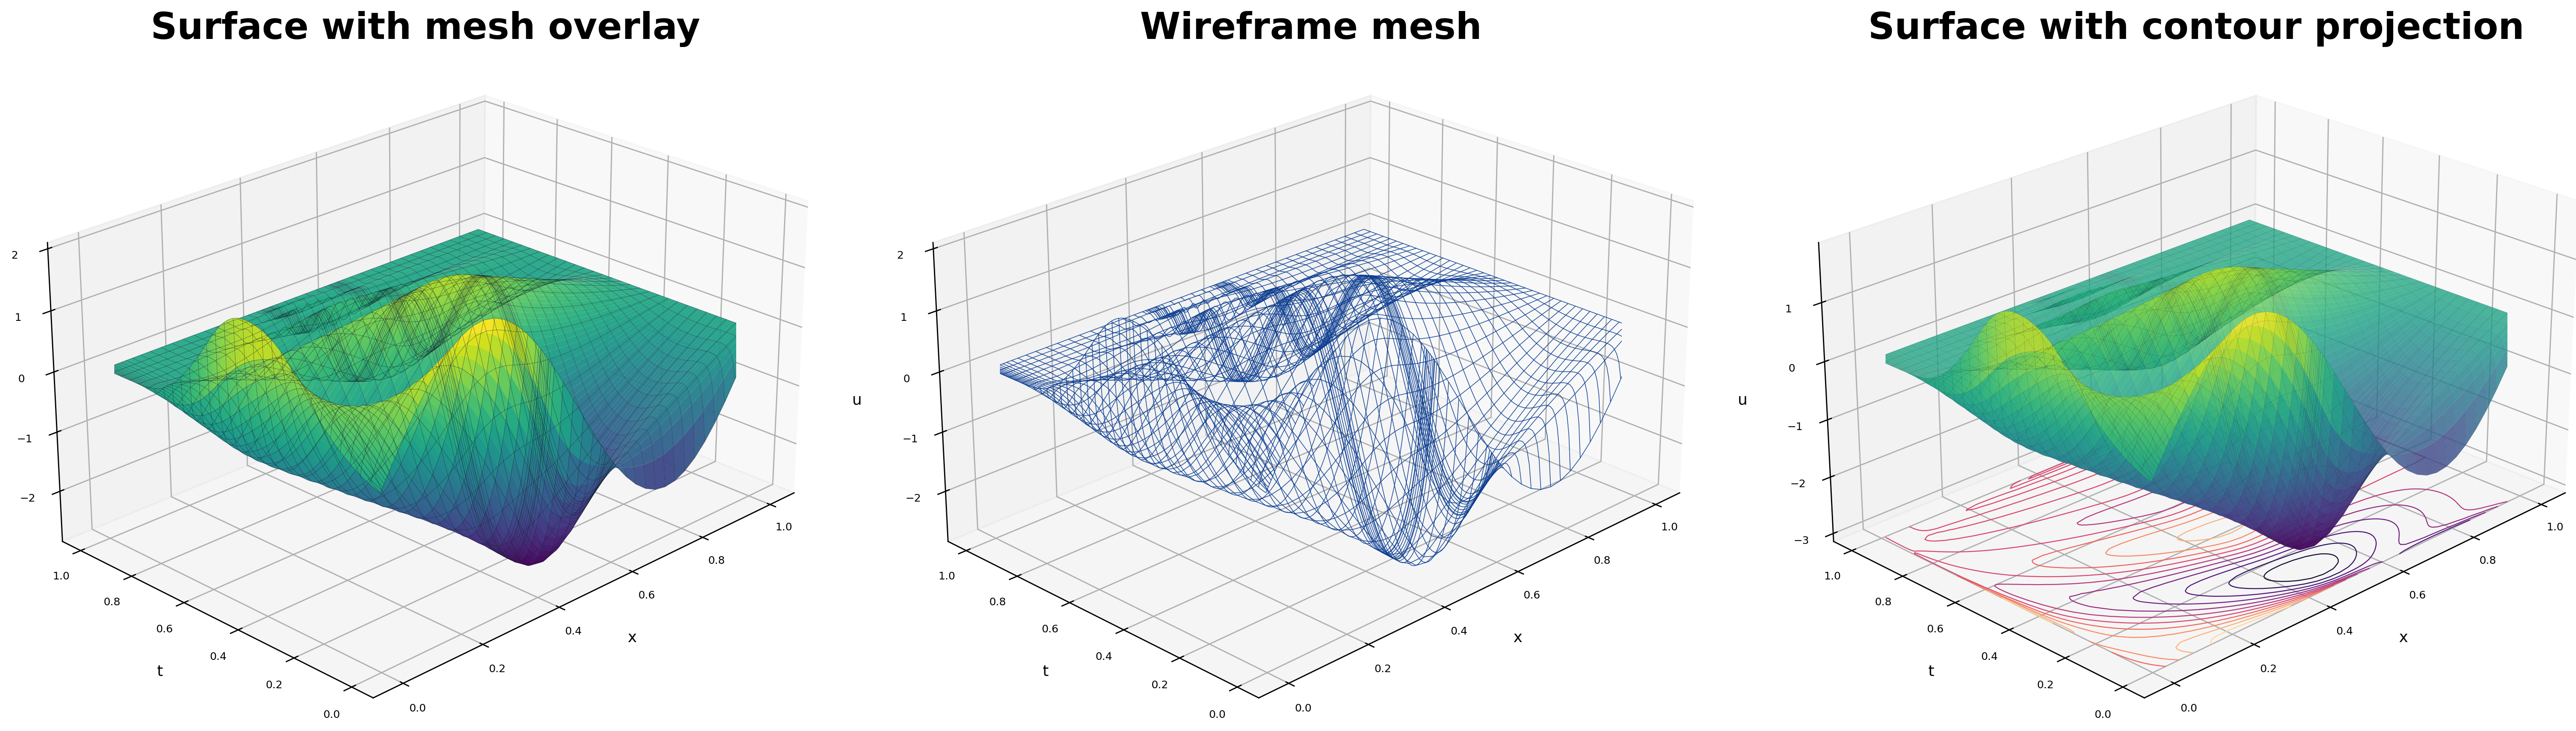
\includegraphics[width=\textwidth,height=0.72\textheight,keepaspectratio,trim=0 18bp 0 0,clip]{degenerate_nonlocal_control_surface_variants.png}
\end{center}

\small
Three views of the same solution: a surface with mesh edges, a wireframe,
and a surface with contours.

\end{frame}

% --------------------------------------------------------------------------
\section{Optimal control}
% --------------------------------------------------------------------------

\dividerframe{EXAMPLE 10}{Optimal control of a heat equation with drift}

\begin{frame}{Heat equation with drift as a state constraint}

\begin{block}{Distributed source-control problem}
\[
    \min_f
    J(f)
    =
    \frac12\|y(T)-y_T\|_{L^2(\Omega)}^2
    +
    \frac{\alpha}{2}
    \int_0^T \|f(t)\|_{L^2(\Omega)}^2\,dt
\]
subject to
\[
    y_t - \nu\Delta y + \boldsymbol{\beta}\cdot\nabla y = f,
    \quad
    y=0\text{ on }\partial\Omega,
    \quad
    y(0)=y_0.
\]
\end{block}

\medskip
\small
\begin{itemize}
    \item $y$: temperature or concentration.
    \item $\nu\Delta y$: diffusion/smoothing.
    \item $\boldsymbol{\beta}\cdot\nabla y$: drift/advection by a background flow.
    \item $f$: distributed heater, source, or actuator to be optimized.
\end{itemize}

\end{frame}

\begin{frame}{State, adjoint, optimality}

For final-time tracking, the first-order system is
\[
\begin{aligned}
    y_t - \nu\Delta y + \boldsymbol{\beta}\cdot\nabla y &= f,
    && y(0)=y_0,\\
    -p_t - \nu\Delta p - \boldsymbol{\beta}\cdot\nabla p &= 0,
    && p(T)=y(T)-y_T,\\
    \alpha f + p &= 0.
\end{aligned}
\]

\bigskip
\small
\textbf{Workflow:}
\begin{enumerate}
    \item Solve the state equation forward in time.
    \item Solve the adjoint equation backward in time.
    \item Update the source control using the reduced gradient
          $g=\alpha f+p$.
\end{enumerate}

\medskip
With a running tracking term
$\frac12\int_0^T\|y-y_d\|^2dt$, the adjoint gets a source term $y-y_d$.

\end{frame}

\begin{frame}{Why $g=\alpha f+p$?}

For the state produced by the current control $f$, the objective is
\[
    J(f)=\frac12\|y(T)-y_T\|_{L^2(\Omega)}^2
    +\frac{\alpha}{2}\int_0^T\|f(t)\|_{L^2(\Omega)}^2\,dt .
\]

\small
For a perturbation $\delta f$, the state variation $\delta y$ solves the
linearized state equation with right-hand side $\delta f$.  Testing that
linearized equation with the adjoint $p$ and integrating by parts gives
\[
    (y(T)-y_T,\delta y(T))
    =
    \int_0^T (p,\delta f)_{L^2(\Omega)}\,dt .
\]
Therefore
\[
    J'(f)\delta f
    =
    \int_0^T (\alpha f+p,\delta f)_{L^2(\Omega)}\,dt,
    \qquad
    g=\nabla J(f)=\alpha f+p .
\]

\medskip
\scriptsize
One backward adjoint solve gives the whole gradient, regardless of the number
of control variables. Alternatives include finite differences, automatic
differentiation, and a direct solve of the full KKT system.

\end{frame}

\begin{frame}[fragile]{Optimal control loop: key code}

\begin{lstlisting}[basicstyle=\ttfamily\tiny]
controls = [fem.Function(V) for n in range(num_steps)]

for it in range(control_iters):
    # 1. forward state solve
    states = solve_state(y0, controls)

    # 2. backward adjoint solve
    p_T.x.array[:] = states[-1].x.array - target.x.array
    adjoints = solve_adjoint(p_T)

    # 3. reduced-gradient update
    for n, f_n in enumerate(controls):
        gradient = alpha*f_n.x.array + adjoints[n+1].x.array
        f_n.x.array[:] = f_n.x.array - step_size*gradient
\end{lstlisting}

\medskip
\small
Reuse the assembled heat operators. Only the right-hand sides change
during the forward and backward solves.

\end{frame}

\begin{frame}{Optimal control: result}

\begin{center}
    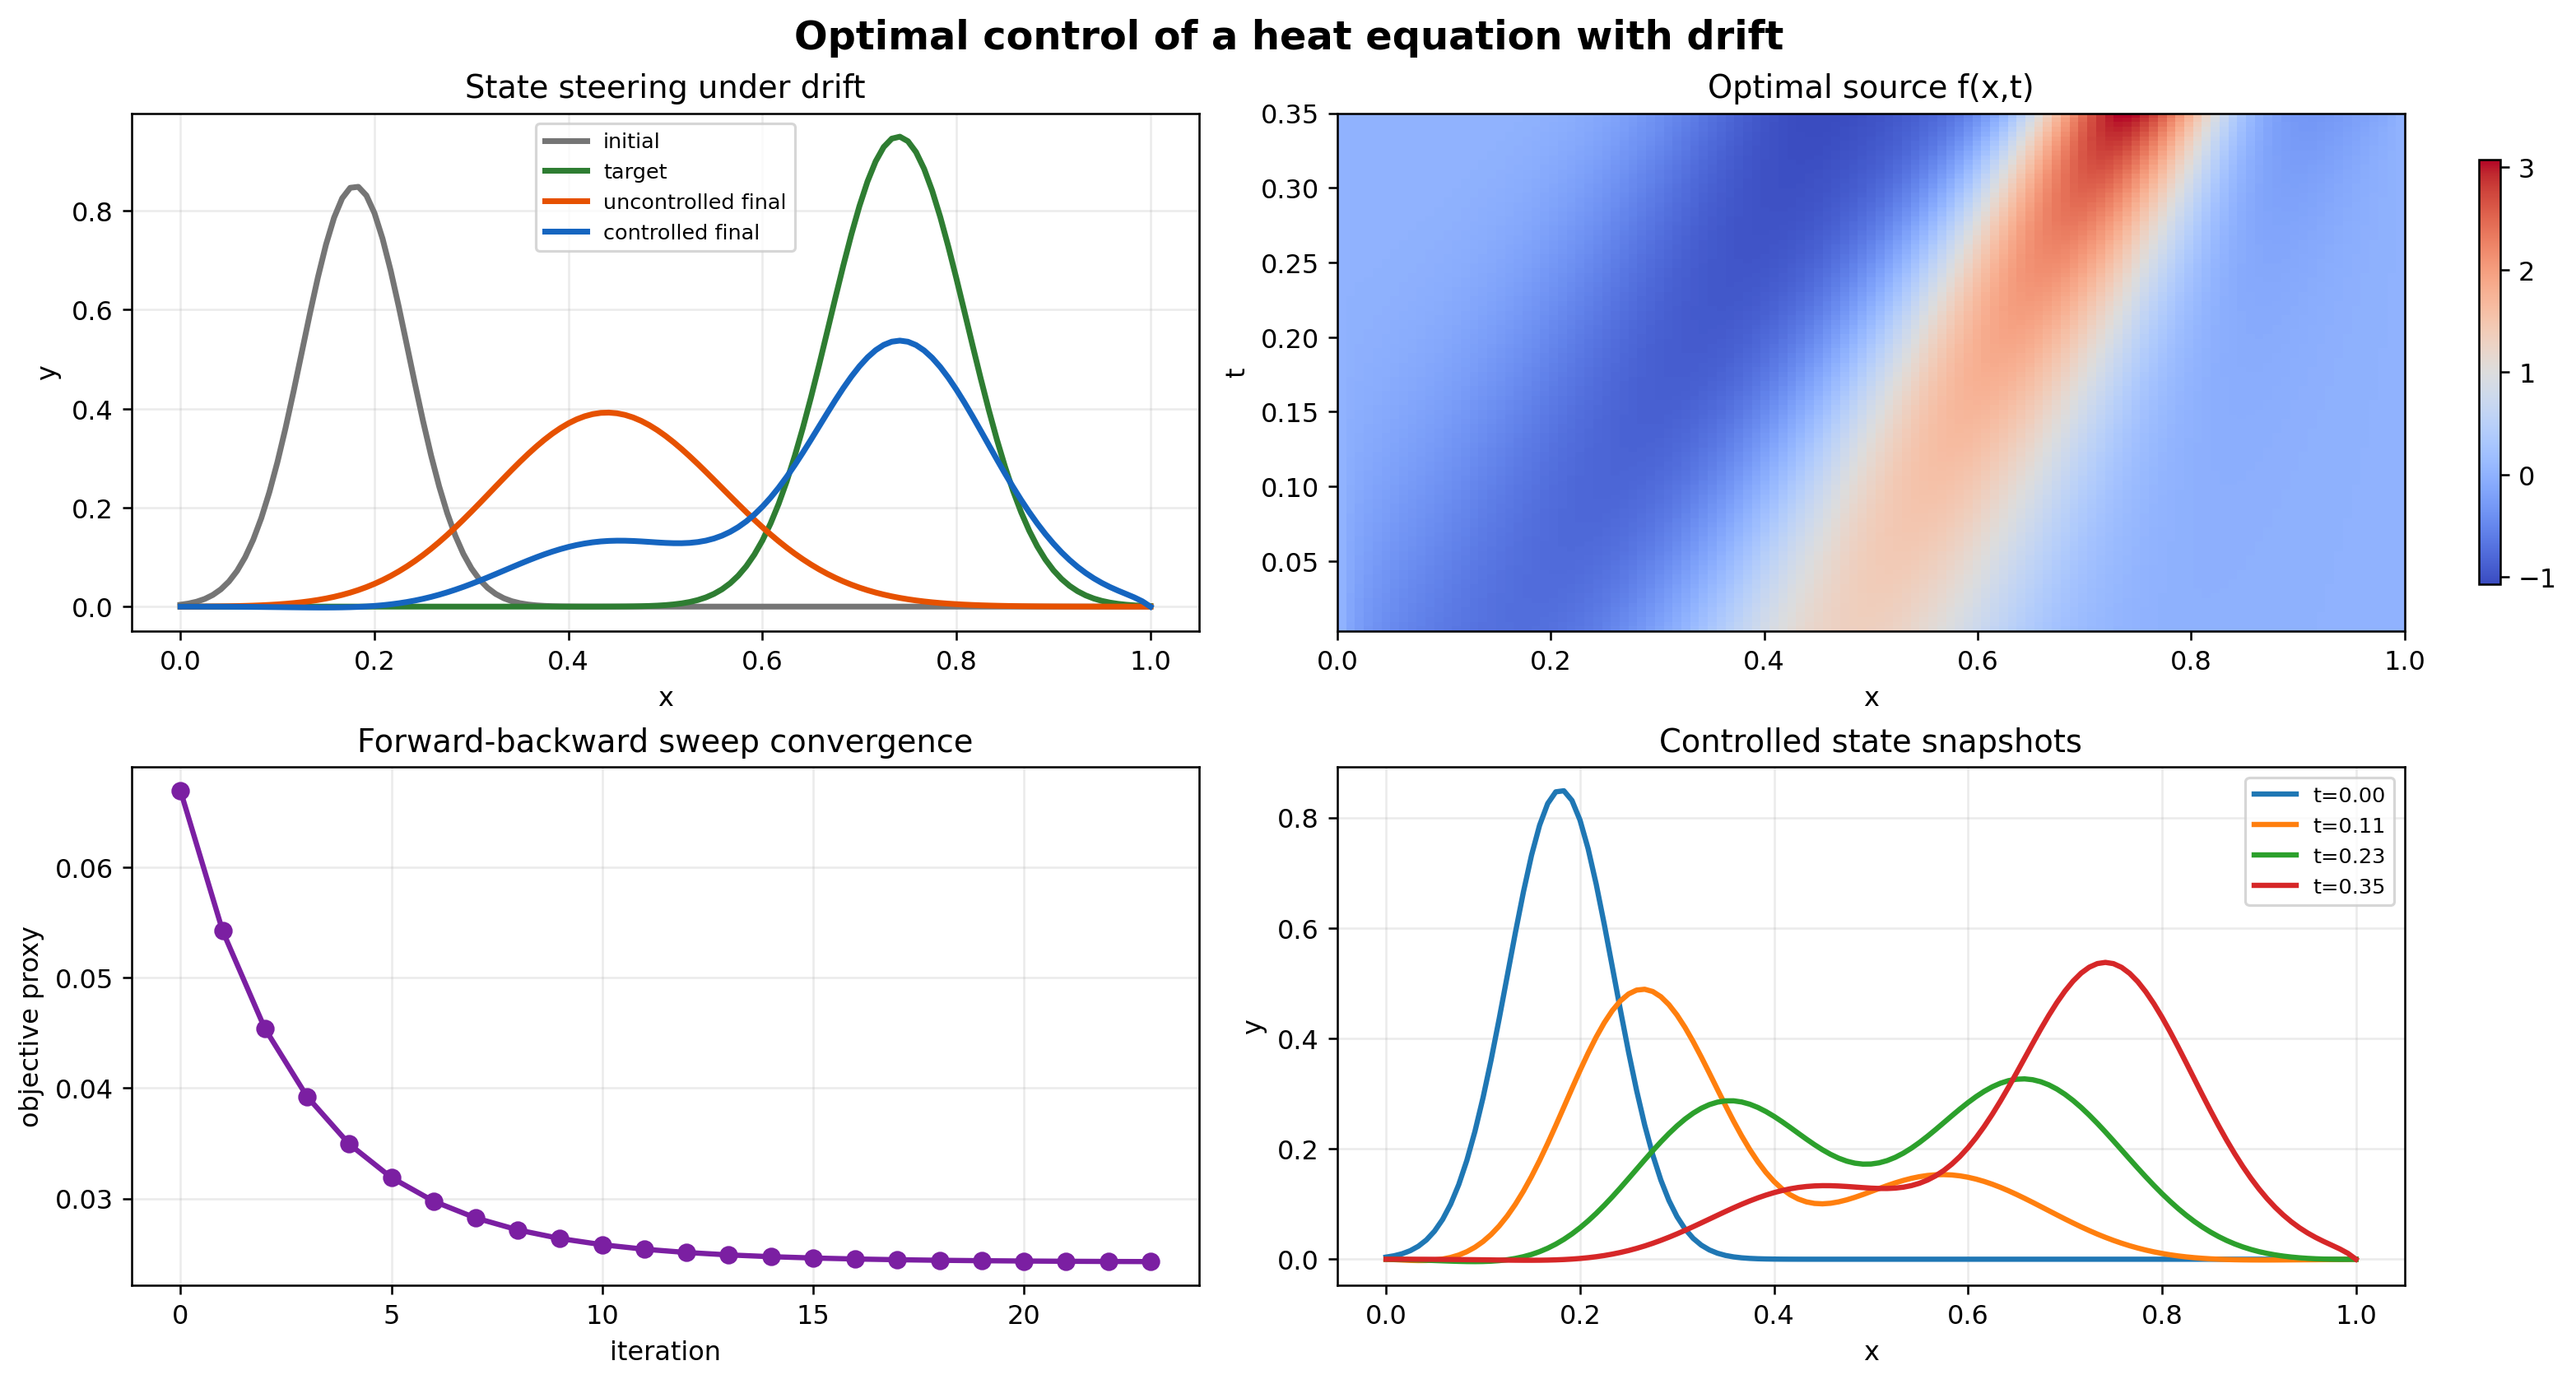
\includegraphics[width=\textwidth,height=0.82\textheight,keepaspectratio]{heat_drift_control.png}
\end{center}

\end{frame}

% --------------------------------------------------------------------------
\section{Coupled reaction-diffusion}
% --------------------------------------------------------------------------

\dividerframe{EXAMPLE 11}{Coupled reaction-diffusion system}

\begin{frame}{Coupled nonlinear reaction-diffusion system}

\begin{block}{Gray-Scott activator-substrate model}
\[
\begin{aligned}
    u_t - D_u\Delta u &= -u v^2 + F(1-u),\\
    v_t - D_v\Delta v &= \phantom{-}u v^2 - (F+k)v,
\end{aligned}
\qquad
\partial_n u=\partial_n v=0.
\]
\end{block}

\medskip
\small
\begin{itemize}
    \item $u$: feed/substrate concentration.
    \item $v$: autocatalytic species concentration.
    \item $uv^2$: nonlinear reaction coupling the two equations.
    \item $F(1-u)$: feed replenishment; $(F+k)v$: removal/decay.
    \item Unequal diffusion and nonlinear reaction can create spatial patterns.
\end{itemize}

\end{frame}

\begin{frame}{Mixed weak form}

Use $W=V\times V$ and test functions $(\phi,\psi)$.
At a backward Euler step, find $(u^{n+1},v^{n+1})\in W$ such that
\[
\begin{aligned}
0=&
\left(\frac{u^{n+1}-u^n}{\Delta t},\phi\right)
+D_u(\nabla u^{n+1},\nabla\phi)
-(-u^{n+1}(v^{n+1})^2+F(1-u^{n+1}),\phi)\\
&+
\left(\frac{v^{n+1}-v^n}{\Delta t},\psi\right)
+D_v(\nabla v^{n+1},\nabla\psi)
-(u^{n+1}(v^{n+1})^2-(F+k)v^{n+1},\psi).
\end{aligned}
\]

\medskip
\small
The homogeneous Neumann condition is natural: no boundary constraint is needed.

\end{frame}

\begin{frame}[fragile,shrink=6]{Reaction-diffusion: FEniCS residual}

\begin{lstlisting}[basicstyle=\ttfamily\tiny]
P1 = basix.ufl.element("Lagrange", msh.basix_cell(), 1)
W = fem.functionspace(msh, basix.ufl.mixed_element([P1, P1]))

w = fem.Function(W)       # current unknown pair
w_old = fem.Function(W)   # previous time level
u, v = ufl.split(w)
u0, v0 = ufl.split(w_old)
phi, psi = ufl.TestFunctions(W)

R_u = -u*v*v + F_feed*(1.0-u)
R_v =  u*v*v - (F_feed+k_kill)*v

F = ((u-u0)/dt)*phi*ufl.dx + D_u*ufl.inner(ufl.grad(u), ufl.grad(phi))*ufl.dx \
    - R_u*phi*ufl.dx \
    + ((v-v0)/dt)*psi*ufl.dx + D_v*ufl.inner(ufl.grad(v), ufl.grad(psi))*ufl.dx \
    - R_v*psi*ufl.dx
J = ufl.derivative(F, w)

problem = NonlinearProblem(F, w, bcs=[], J=J,
    petsc_options={"snes_type": "newtonls",
                   "ksp_type": "preonly", "pc_type": "lu"})

for step in range(num_steps):
    problem.solve()
    w_old.x.array[:] = w.x.array
\end{lstlisting}

\end{frame}

\begin{frame}{Reaction-diffusion: pattern formation}

\begin{center}
    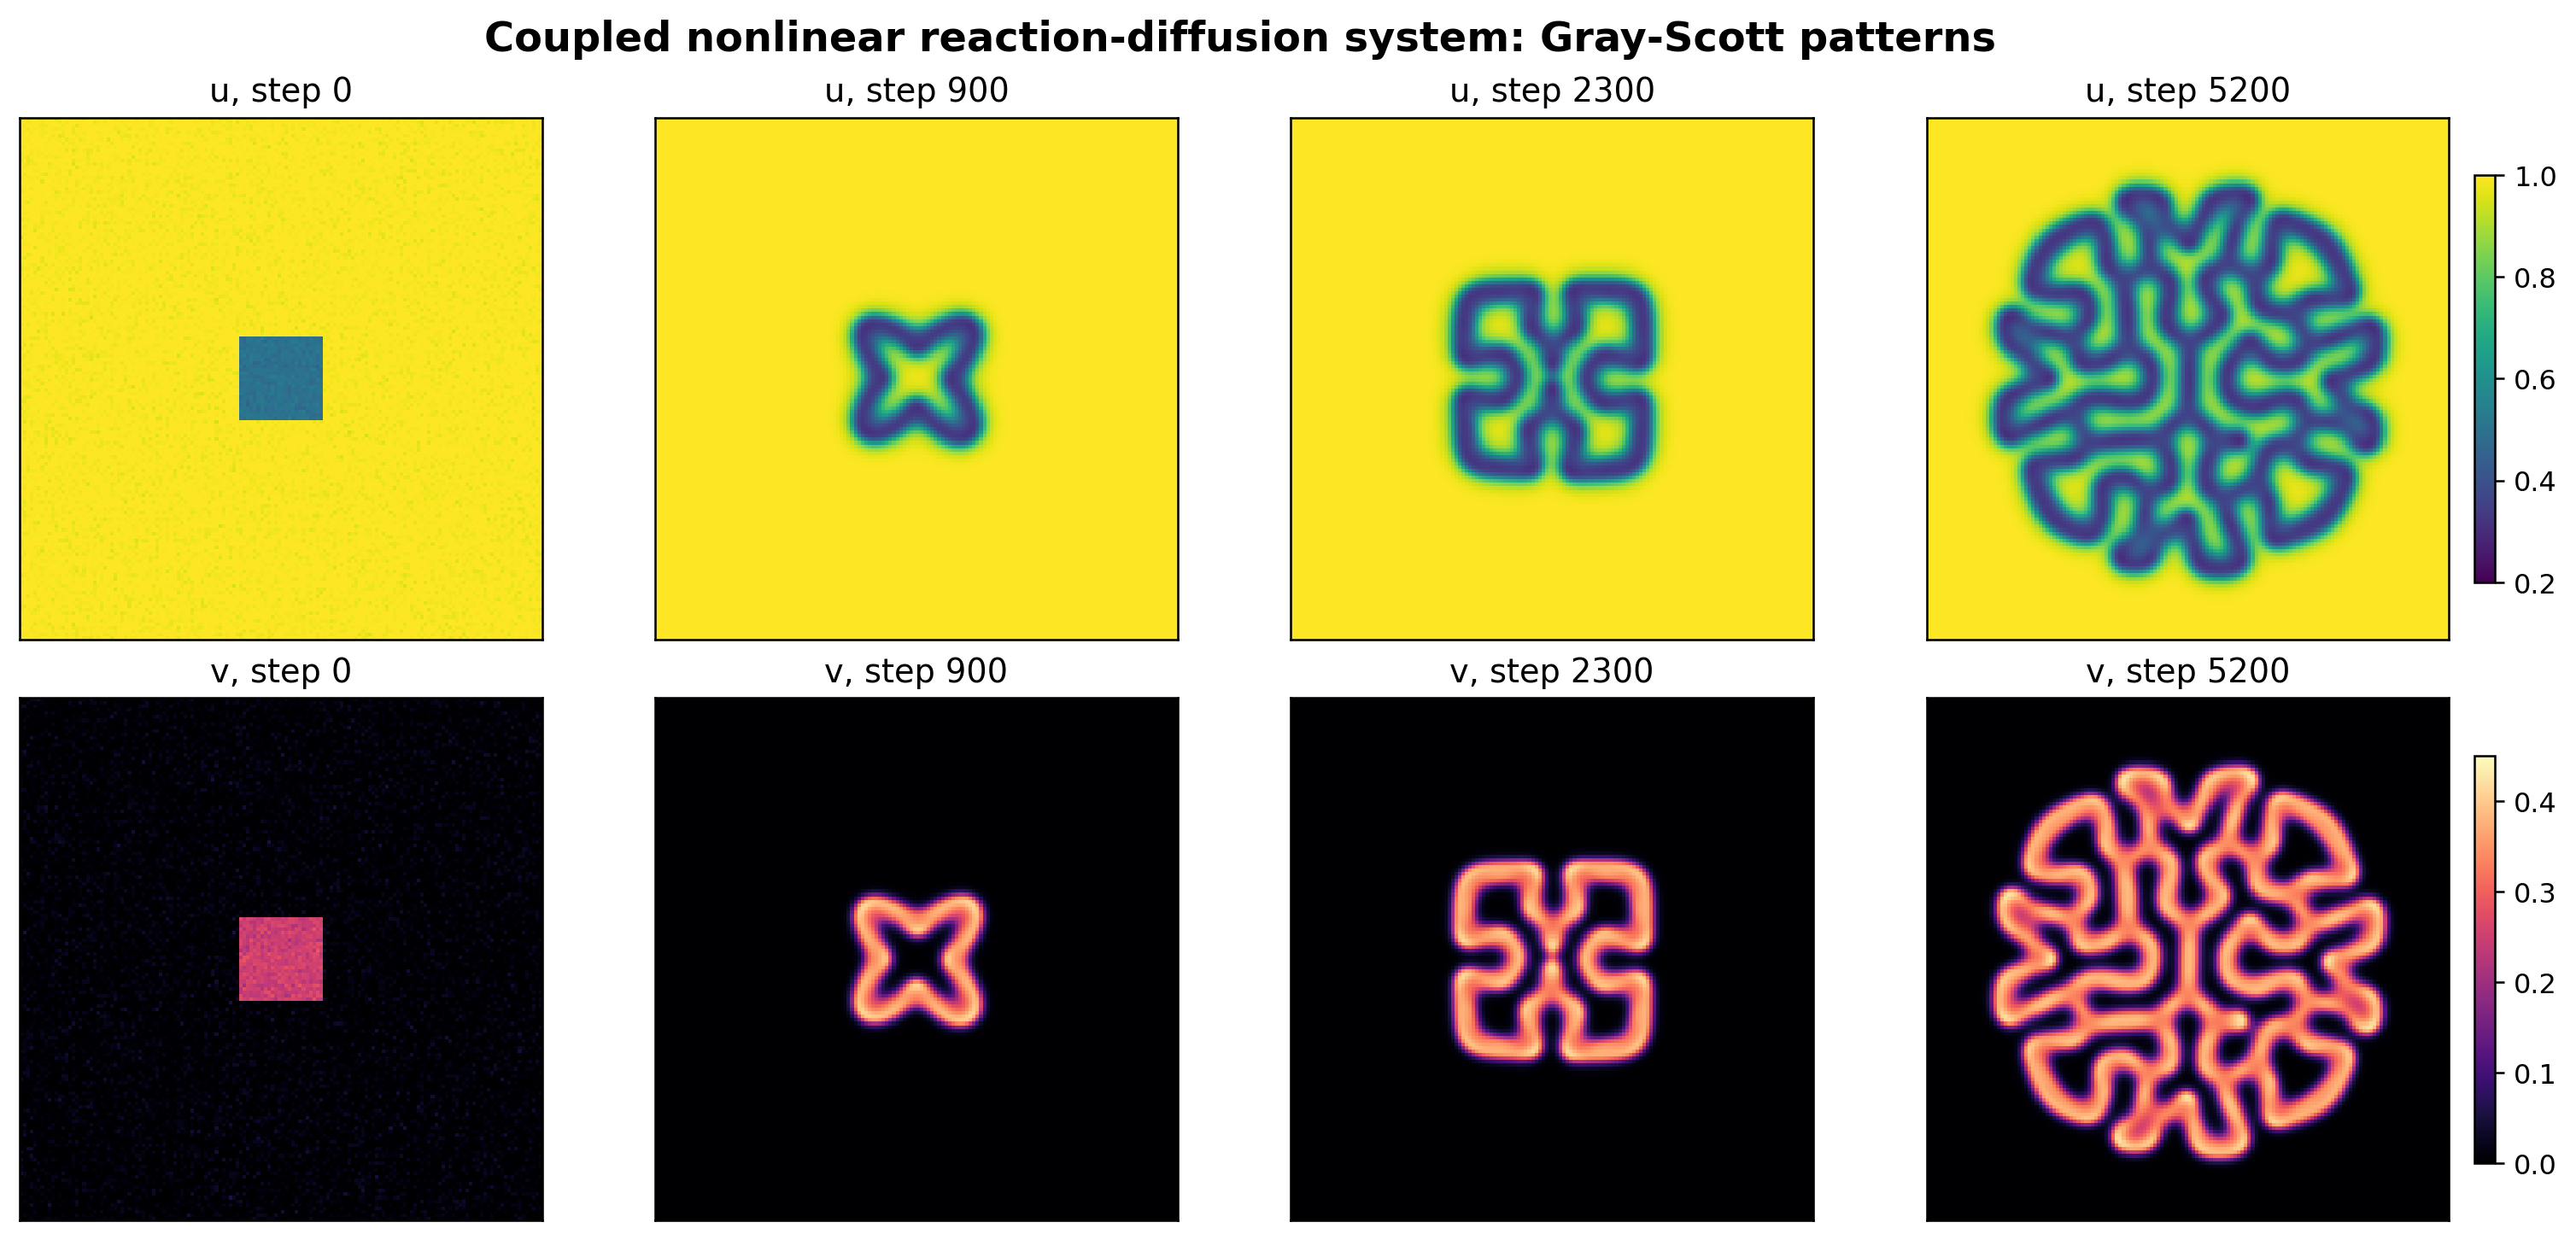
\includegraphics[height=0.64\textheight]{reaction_diffusion_system.png}
\end{center}

\small
The nonlinearity transfers mass between the two species while diffusion spreads
each species at a different rate. Together they produce the patterns shown here.

\end{frame}

% --------------------------------------------------------------------------
\section{Summary}
% --------------------------------------------------------------------------

\begin{frame}{Solving the five problem types}

\begin{itemize}
    \item Nonlinear PDEs: write $F(u;v)=0$ and let UFL differentiate the Jacobian.
    \item Nonlocal PDEs: assemble global quantities, then solve linearized steps.
    \item Degenerate control problems: combine linearized controllability maps with adjoint refinement.
    \item Optimal control: solve the state forward and the adjoint backward to compute the gradient.
    \item Coupled systems: use mixed spaces and solve for all fields together.
\end{itemize}

\end{frame}

\dividerframe{}{Questions?}

\appendix

\begin{frame}[fragile]{Backup: rebuild figures}

\begin{lstlisting}[language=bash, basicstyle=\ttfamily\tiny]
conda run -n fenicsx-env python experiments/10_plaplacian_3d.py
conda run -n fenicsx-env python experiments/11_nonlocal_variants.py
python experiments/14_degenerate_nonlocal_control.py --mesh feature --nx 60 --nt 120 --refine-iters 50
conda run -n fenicsx-env python experiments/12_heat_drift_control.py
conda run -n fenicsx-env python experiments/13_reaction_diffusion_system.py
\end{lstlisting}

\medskip
\small
Compile the deck:
\begin{lstlisting}[language=bash, basicstyle=\ttfamily\tiny]
latexmk -pdf -interaction=nonstopmode 1.2_fenics_part2.tex
\end{lstlisting}

\end{frame}

\end{document}
